\chapter{Sortida del planeta origen}
Un cop es disposa dels elements keplerians eclíptics de l'òrbita de transferència, és possible trobar tant la trajectòria el·líptica que la sonda haurà de prosseguir des de la seva òrbita d'aparcament fins la sortida de l'EdI, com el $\Delta V$ que se li haurà d'aplicar per a que sigui capaç d'arribar al planeta en el temps marcat.

\begin{figure}[H]
	\centering
	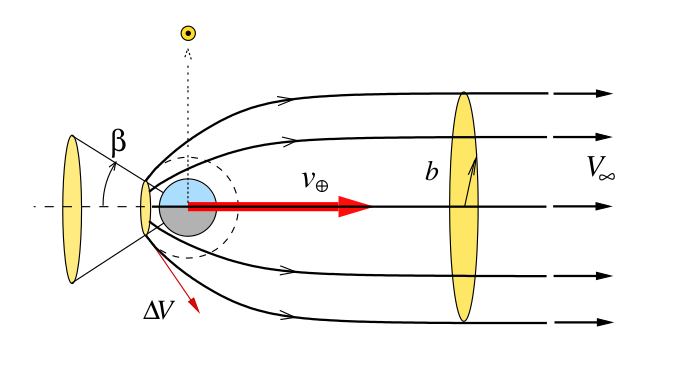
\includegraphics[scale=0.5]{./plots/hyperbola}
	\caption{Òrbita hiperbòlica de sortida de l'esfera d'influència del planeta.}
	\label{esquema_hyperbola}
\end{figure}
A la figura \ref{esquema_hyperbola} es veuen els elements rellevants que s'han d'obtenir.
\section{Velocitats a la sortida}
El primer que cal trobar són les velocitats $V_inf$ i $V_1$, planetocèntrica i heliocèntrica respectivament, de la sonda al moment de sortida de l'EdI del planeta. Això es fa..........
AQUI JM! Pots fer referencia a \ref{OrbitalVectors}

\section{Òrbita planetocèntrica hiperbòlica}
A les classes de l'assignatura s'ha arribat a les següents relacions \cite{Calaf2017d}:
\begin{equation}
a = \frac{\mu}{V_{\infty}^{2}}
\end{equation}
\begin{equation}
e = 1 + \Big(\frac{V_{\infty}}{V_{o}}\Big)^2
\end{equation}
\begin{equation}
\cos(\beta) = \frac{1}{e}
\end{equation}
\begin{equation}
b = a\sqrt{e^2-1}
\end{equation}
\begin{equation}
V_o = \sqrt{\frac{\mu}{r_o}}
\end{equation}
On:
\begin{itemize}
	\item a és el semieix major.
	\item e és l'excentricitat.
	\item $\beta$ és l'angle de l'asímptota. Veure fig.\ref{esquema_hyperbola}.
	\item b és el paràmetre de sortida. Veure fig.\ref{esquema_hyperbola}.
	\item $V_o$ és la velocitat que porta la sonda en l'òrbita d'aparcament de radi $r_o$.
	\item $\mu$ és el paràmetre de gravitació estàndard del planeta. (GM)
	\item $V_{\infty}$ representa el mòdul de la velocitat planetocèntrica que porta la sonda al sortir del planeta.
\end{itemize}
Aquests càlculs s'han portat a terme mitjançant el codi de la secció \ref{outHyperbola}.
\section{DeltaV}
Per trobar l'impuls que s'ha de subministrar s'aplica conservació d'energia cinètica:
\begin{equation*}
\frac{1}{2}V_{\infty}^2 =\frac{1}{2}(V_o + \Delta V)^2 - \frac{\mu}{r_o}
\end{equation*}
Arribant així a:
\begin{equation}
\Delta V = \sqrt{V_{\infty}^2+2V_{o}^2} - V_o
\end{equation}
